\input information.tex
\usepackage{geometry}  %Set the size of each part of the page
\usepackage{fancyhdr}  %Set header, margin and footer
\usepackage{pifont}  %Special symbol font
\usepackage{graphicx}  %For illustration
\usepackage{ctex} %for Chinese
\usepackage{placeins} %\FloatBarries
\usepackage{extramarks}  %extra marks
\usepackage{mathrsfs} %Mathematical font
\usepackage{mathtools} %Mathematical tools
\usepackage{amsmath}  %Mathematical formula
\usepackage{amssymb}  %Mathematical fonts and symbols
\usepackage{amsthm} %Mathematical theorem format control
\usepackage{tikz} %Draw
\usepackage{algorithm} %algorithm
\usepackage{algpseudocode} %algpseudo code
\usepackage{tabularx} %Automatic calculation of column width
\usepackage{setspace} %Set space
\usepackage[framed,numbered,autolinebreaks,useliterate]{mcode} %Insert code
\usepackage{paralist} %Reduce the gap for itemize and enditemize
\usepackage[parent]{currfile}
\usepackage{listings}
\usepackage{url}
\usepackage{xstring}
\usepackage[colorlinks, linkcolor=black, anchorcolor=black, citecolor=black, ]{hyperref}
\usepackage{xparse}
\usetikzlibrary{positioning, fit, calc, intersections, through, shapes, arrows, scopes, automata, decorations.markings}
\newtheorem{lemma}{Lemma}
\newtheorem{theorem}{Theorem}
\newtheorem{remark}{Remark}
\newtheorem{corollary}{Corollary}
\renewcommand{\proofname}{\bf Proof}
\renewcommand{\thesection}{}
\let\itemize\compactitem 
\let\enditemize\endcompactitem 
\let\enumerate\compactenum 
\let\endenumerate\endcompactenum 
\let\description\compactdesc 
\let\enddescription\endcompactdesc
\theoremstyle{plain}% default

%
% Basic Document Settings
%

\CTEXoptions[today=old]

\topmargin=-0.45in
\evensidemargin=0in
\oddsidemargin=0in
\textwidth=6.5in
\textheight=9.0in
\headsep=0.25in

\linespread{1.3}

\pagestyle{fancy}
\lhead{\hmwkAuthorName}
\chead{\hmwkClass\ : \hmwkTitle}
\rhead{\firstxmark}
\lfoot{\lastxmark}
\cfoot{\thepage}

\renewcommand\headrulewidth{0.4pt}
\renewcommand\footrulewidth{0.4pt}

\setlength\parindent{2em}

%
% Create Problem Sections
%

\newcommand{\enterProblemHeader}[1]{
    \nobreak\extramarks{}{Problem \arabic{#1} continued on next page\ldots}\nobreak{}
    \nobreak\extramarks{Problem \arabic{#1} (continued)}{Problem \arabic{#1} continued on next page\ldots}\nobreak{}
}

\newcommand{\exitProblemHeader}[1]{
    \nobreak\extramarks{Problem \arabic{#1} (continued)}{Problem \arabic{#1} continued on next page\ldots}\nobreak{}
    \stepcounter{#1}
    \nobreak\extramarks{Problem \arabic{#1}}{}\nobreak{}
}

\setcounter{secnumdepth}{0}
\newcounter{partCounter}
\newcounter{homeworkProblemCounter}
\setcounter{homeworkProblemCounter}{1}
\nobreak\extramarks{Problem \arabic{homeworkProblemCounter}}{}\nobreak{}

\newenvironment{homeworkProblem}{
    \section{Problem \arabic{homeworkProblemCounter}}
    \setcounter{section}{\arabic{homeworkProblemCounter}}
    \setcounter{partCounter}{1}
    \enterProblemHeader{homeworkProblemCounter}
}{
    \exitProblemHeader{homeworkProblemCounter}
}


%
% Create jobname
%

\newcommand*{\myjobname}{}
\newcommand*{\setmyjobname}{%
  \edef\myjobname{\jobname}%
  \expandafter\expandafter\expandafter\setmyjobnameaux
    \expandafter\myjobname\expandafter"\myjobname"\relax
}
\newcommand*{\setmyjobnameaux}{}
\def\setmyjobnameaux#1"#2"#3\relax{\def\myjobname{#2}}
\setmyjobname


\makeatletter
\catcode`\_=12
\newcommand{\filenameparse}[1]{\expandafter\filename@parse@#1\@nil}
\def\filename@parse@#1_#2_#3\@nil{%
  \gdef\fileA{#1}% first part
  \gdef\fileB{#2}% middle part
  \gdef\fileC{#3}% final part
}
\catcode`\_=8
\makeatother
\filenameparse{\myjobname}

%
% Title Page
%

\title{
    \vspace{0.5in}
    \textmd{\textbf{\hmwkClass: \hmwkTitle}}\\
    \normalsize\vspace{0.1in}\small{Finished\ on\ \hmwkDueDate\ }\\
   \vspace{0.1in}\large{\textit{\hmwkClassInstructor}}
    \vspace{3in}
\FloatBarrier
\begin{figure}[htb] 
\center{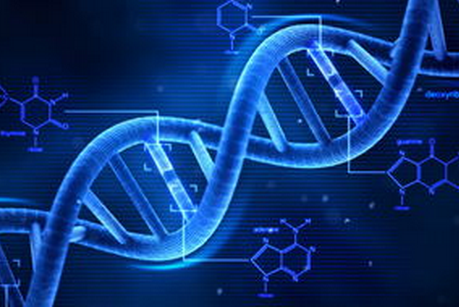
\includegraphics[width=5cm]  {DNA.png}} 
\end{figure}
 \FloatBarrier
 \author{\textbf{\hmwkAuthorName}}
\date{\hmwkStudentID}
}


%
% Various Helper Commands
%

% Alias for the Solution section header
\newcommand{\solution}{\par   \noindent   \textbf{Solution}\\ \indent}
\newcommand{\Solution}{\par   \noindent   \textbf{Solution}}

% Probability commands: Expectation, Variance, Covariance, Bias and so on.
\newcommand{\E}{\mathrm{E}}
\newcommand{\Var}{\mathrm{Var}}
\newcommand{\Cov}{\mathrm{Cov}}
\newcommand{\Bias}{\mathrm{Bias}}
\newcommand{\alg}[1]{\textsc{\bfseries \footnotesize #1}}
\newcommand{\deriv}[1]{\frac{\mathrm{d}}{\mathrm{d}x} (#1)}
\newcommand{\pderiv}[2]{\frac{\partial}{\partial #1} (#2)}
\newcommand{\dx}{\mathrm{d}x}
\renewcommand{\part}[1]{\textbf{\large Part \Alph{partCounter}}\stepcounter{partCounter}\\}

\makeatletter
\def\picfour#1#2#3#4{
\FloatBarrier
\begin{figure}[htb] 
\center{\includegraphics[width=#2]  {#1}} 
\caption{#3}
\label{#4}
\end{figure}
\FloatBarrier
}
\def\picthree#1#2#3{
\FloatBarrier
\begin{figure}[htb] 
\center{\includegraphics[width=#2]  {#1}} 
\caption{#3}
\end{figure}
\FloatBarrier
}
\def\pictwo#1#2{
\FloatBarrier
\begin{figure}[htb] 
\center{\includegraphics[width=#2]  {#1}} 
\end{figure}
\FloatBarrier
}
\makeatother 
\NewDocumentCommand{\pic}{mmgg}{
\IfDecimal{#2}{%
    {\IfNoValueTF{#4}
    {\IfNoValueTF{#3}
    {\pictwo{#1}{#2\textwidth}}
    {\picthree{#1}{#2\textwidth}{#3}}
    }
    {\picfour{#1}{#2\textwidth}{#3}{#4}}}
    }{%
     {\IfNoValueTF{#4}
    {\IfNoValueTF{#3}
    {\pictwo{#1}{#2}}
    {\picthree{#1}{#2}{#3}}
    }
    {\picfour{#1}{#2}{#3}{#4}}}
    }%
}


